\section{Test der Batterie}
Die Batterie konnte durch diverse Tests auf ihre Funktionstüchtigkeit geprüft werden. Dazu gehört ebenfalls die Steuerplatine, da diese die Informationen von und zur Batterie verarbeitet. Das BMS selbst wurde dabei nicht getestet, da diese Tests bereits vom Hersteller durchgeführt wurden. Es wurde lediglich die korrekte Funktion an der Batterie überprüft.

\subsection{Steuerplatine}
Um die korrekte Funktion der Steuerplatine sicherzustellen, wurde diese in drei Schritten aufgebaut. Als erstes wurde die Schaltung aufgebaut und im Simulationsprogramm LtSpice überprüft. Anschliessend wurde ein Prototyp gebaut, an welchem die Signale eingespeist und die Ausgänge vermessen wurden. Als auch dies funktionierte, wurde eine Platine bestellt, welche nach der Bestückung ebenfalls getestet wurde.

Da die einzelnen Schaltungspfade gut voneinander trennbar sind, konnten sie einzeln getestet werden. Dabei wurden die folgenden Punkte überprüft: \begin{itemize}
	\item Die $12$ V-Einspeisung wird beim Anschluss von $230$ VAC unterbrochen
	\item An den Einschalt-Anschlüssen liegt bei vorhandener Speisespannung die korrekte Spannung an
	\item Beide Ladegeräte können einzeln ein- und ausgeschaltet werden
	\item Der Hauptschalter wird nur eingeschaltet, wenn beide BMS dies erlauben
	\item Die Lüftergruppen können einzeln ein- und ausgeschaltet werden
	\item Am Ladezustandsausgang liegt immer die kleinere der beiden Spannungen an
	\item Das BMS wird auch während dem Ladevorgang mit Spannung versorgt
	\item Der Anschluss von $230$ VAC wird an das BMS übermittelt
\end{itemize}

Durch diese Tests konnte sichergestellt werden, dass die Steuerplatine wie gewünscht funktioniert. Dabei mussten jedoch Anpassungen gemacht werden, da zuerst davon ausgegangen wurde, dass das Batteriemanagementsystem mit einer Spannung von $24$ VDC arbeitet. Da dies jedoch, aufgrund einer anderen Bezugsquelle, noch geändert hat, wurde der $24$ V Spannungswandler überbrückt.

\subsection{Einzelzellen}
Um Fehler von Beginn an zu realisieren, wurden vor der Verschaltung die einzelnen Zellen getestet. Zu diesem Zweck wurde an jeder Zelle die Spannung gemessen. Da die Zellen vorgängig alle komplett geladen waren wäre eine defekte Zelle durch eine niedrigere Spannung aufgefallen.

Damit die einzelnen Zellen, die jeweils parallel geschaltet werden, beim Zusammenhängen keine grossen Ströme fliessen lassen, wurden diese über eine längere Zeit mit $1\ \Omega$-Widerständen ausgeglichen. Dadurch wurden die Ausgleichsströme begrenzt und die Spannungen der Zellen konnten sich langsam angleichen.

\subsection{Zellenverschaltung}
Die Zellenverschaltung an sich ist sehr einfach, wodurch auch die entsprechenden Tests einfach wurden. Es wurde überprüft, ob die Batterien die korrekte Spannung haben. Ausserdem wurde bereits vorgängig an Einzelzellen überprüft, ob sich diese bei starker Belastung erwärmen, was jedoch nicht nachgewiesen werden konnte.

Nach dem Einbau ins Gehäuse wurden sämtliche Anschlüsse auf ihren Sitz überprüft, anschliessend erfolgte eine optische Prüfung nach dem Vier-Augen-Prinzip. Die bei diesen Vorgängen gefundenen Fehler wurden sofort behoben.

Die Funktion des Ladegeräts wurde ebenfalls getestet, indem eine Batterie über einen Lastwiderstand entladen wurde. Dabei wurde bewusst eine ungleichmässige Entladung durchgeführt, um ebenfalls die Balancierfunktion beim anschliessenden Ladeprozess zu überprüfen. Erst danach wurden die Batterien ins Fahrzeug eingebaut.

\color{blue}Für den Test wurde ein Aufbau gemäss Abbildung \ref{fig:Testaufbau} gewählt. Wie man sofort erkennt, ist dabei nur eine Batterie vorhanden. Dies wurde so gewählt, da beide Batterien unabhängig voneinander betrieben werden sollten, also auch keinen Einfluss auf einander haben. Die Wahl einer Batterie vereinfachte ausserdem die Abführung der Leistung über einen Lastwiderstand (für den maximalen Strom beträgt die Leistung bei vollgeladener Batterie immerhin \linebreak$12\cdot4.2$ V $\cdot 150$ A$=7\ 560$ W).\newpage

\begin{figure}[h]
	\centering
		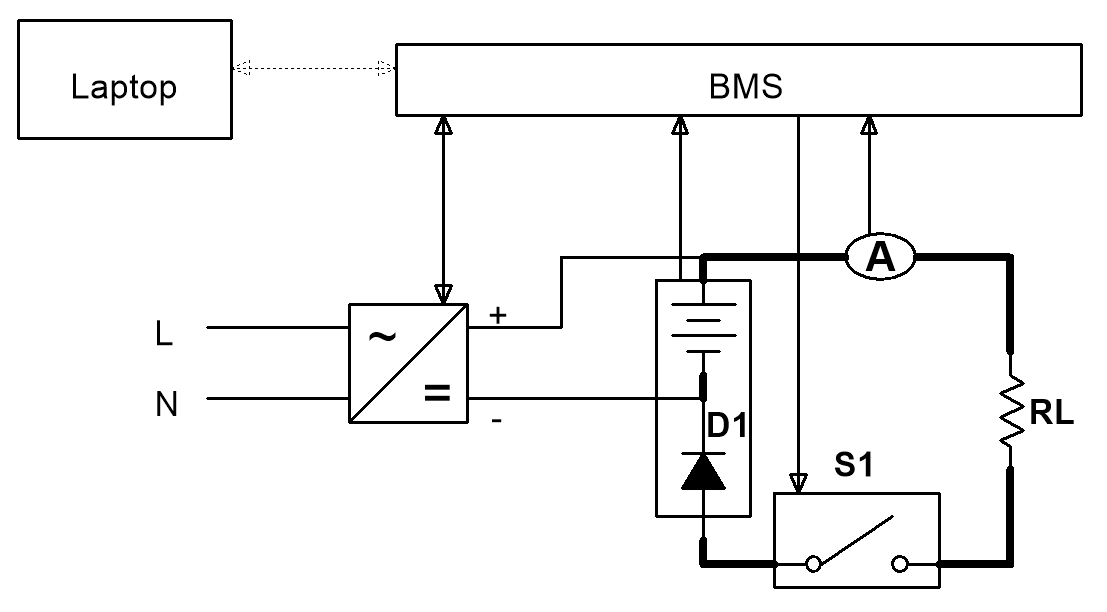
\includegraphics[width=.80\textwidth]{images/Testaufbau.png}
	\caption{Testaufbau für den Test einer Einzelbatterie}
	\label{fig:Testaufbau}
\end{figure}

Der folgende Abschnitt zeigt die Tests, welche ausgeführt wurden, unterteilt in verschiedene Kategorien. Dahinter steht jeweils \textit{kursiv}, welches Resultat erwartet und erhalten wurde. Dabei wurde die Testreihe prinzipiell für die beiden Batterien wiederholt, wobei viele Tests nur für eine Batterie durchgeführt werden mussten, da damit eher die Schaltung als die Batterie selbst getestet wurden.

\paragraph{Sicherheit:} \begin{itemize}
	\item Der Not-Aus wird im Betrieb betätigt: \textit{Das $12$ V-Netz fällt aus, wodurch der Hauptschalter die Stromzufuhr zur Last unterbricht. Dies ist so eingetreten.}
	\item Eine Batterieerwärmung wird mit einem Föhn simuliert: \textit{Zuerst sollten sich die Lüfter einschalten, um die Kühlung der Batterie zu verbessern. Hilft dies nicht (weitere Erhitzung mit dem Föhn), so sollte die Last ausgeschaltet werden. Nach einigen Sekunden schalteten die Lüfter ein, bei weiterer Erwärmung wurde die Stromzufuhr unterbrochen.}
	\item Mit einer Wärmebildkamera wird die Batterie unter Last untersucht: \textit{Warme Stellen, welche auf schlechte Kontakte hindeuten, fallen auf. Es wurde keine solche Stellen gefunden, lediglich die Diode erwärmt sich bei höheren Strömen um ca. $25^\circ$C über Umgebungstemperatur.}
	\item Über einen alten Schütz wird ein Kurzschluss mit möglichst geringem Widerstand simuliert, wobei eine Zerstörung des Schützes bewusst in Kauf genommen wird: \textit{Die Sicherung als Verschleissteil kann den Kurzschluss auslöschen. Die Sicherung verursachte keinerlei Probleme und unterbrach den Stromkreis bevor ein anderes Bauteil zerstört wurde.}
\end{itemize} \newpage

\paragraph{Schaltung:} \begin{itemize}
	\item Das $230$ VAC-Netz wird angeschlossen: \textit{Das $12$ VDC-System fällt - ausser beim BMS - aus. Folglich wird auch der Hauptschalter geöffnet. Die Last wurde ausgeschaltet, während das BMS weiterarbeitete.}
	\item Das alte Voltmeter der Batterie wird angeschlossen: \textit{Die Anzeige der verbleibenden Ladung ist proportional zur verbleibenden Batteriekapazität. Dies wurde so bestätigt.}
	\item Eine Überlast im $12$ VDC-Netz wird simuliert: \textit{Es muss bekannt sein, welche Auswirkungen dies hat. Fällt evt. der Hauptschalter aus? Eine Überlastung führt zu einem Verringern der Ausgangsspannung. Jedoch konnte nicht einmal mit allen eingeschalteten $12$ V-Verbrauchern im Fahrzeug ein genügend grosser Spannungsabfall für den Ausfall von Komponenten bewerkstelligt werden.}
	\item Die Temperatur des Diodengehäuses wird unter Volllast gemessen, um damit einen Rückschluss auf die Diodentemperatur zu ziehen: \textit{Bei zu hoher Temperatur wird ein zusätzlicher Lüfter für den Diodenkühlkörper montiert. Die Diode erwärmt sich bei Volllast um ca. $25^\circ$ C über Umgebungstemperatur und ist noch weit von der Maximaltemperatur entfernt, weshalb kein Lüfter nötig ist.}
	\item Unter Volllast (inklusive Induktivität) wird der Hauptschalter geöffnet: \textit{Eine saubere Abschaltung muss in jedem Fall garantiert sein, auch mit einer induktiven Last wie sie ein Motor darstellt. Der Hauptschalter öffnete ohne Probleme.}
	\item Die Batterie wird nach einer Ladung komplett entladen: \textit{Der im Batteriemanagementsystem ausgelesene Kapazitätswert gibt an, welche reale Kapazität mit den gesetzten Spannungsgrenzen verfügbar ist. Die Batteriekapazität beträgt ungefähr die Hälfte der ursprünglichen Erwartung. Für genauere Details wird auf Abschnitt \ref{sec:ah} verwiesen.}
\end{itemize}

\paragraph{Batteriemanagement-System:} \begin{itemize}
	\item Vor dem Ladevorgang wird eine einzelne Zelle etwas tiefer entladen: \textit{Das Batteriemanagementsystem stellt die gleichmässige Ladung aller Zellen mittels Balancing wieder her. Dieser Vorgang fand so statt, dauert allerdings sehr lange, weshalb dieser Parameter im BMS nachträglich angepasst wurde. Das konnte so durch die Testfahrten verifiziert werden.}
	\item Das Ende des Ladezyklus wird erfasst: \textit{Das Batteriemanagementsystem verhindert ein Überladen der Zellen. Das Ladegerät wurde vom BMS ausgeschaltet.}
	\item Die Batterie wird möglichst tief entladen: \textit{Das Batteriemanagementsystem öffnet den Hauptschalter, um so eine Tiefentladung der Batterie zu verhindern. Dieses Verhalten wurde bestätigt.}
\newpage
	\item Überprüfung der Spannungs- und Strommessung: \textit{Die Genauigkeit dieser Messung, welche vorab als genügend genau angenommen werden kann, wird überprüft, um spätere Fehler von vornherein ausschliessen zu können. Die Messungen weisen im Vergleich zu anderen Messmethoden keine grossen Unterschiede auf.}
	\item Nach den Tests wird das Batteriemanagementsystem mit dem Computer verbunden: \textit{Die ausgelesenen Daten werden auf Plausibilität hin überprüft. Sämtliche Daten erscheinen plausibel.}
\end{itemize}\color{black}


\newpage